% !TEX encoding = UTF-8
% !TEX TS-program = pdflatex
% !TEX root = ../tesi.tex

%**************************************************************
\chapter{Architettura generale ed analisi container}
\label{cap:architettura-progetto-container}
%**************************************************************

\intro{Breve introduzione al capitolo}\\
In questo capitolo si esporrà l'architettura generale del progetto implementata in Azienda, fornendo un'analisi dettagliata sulla composizione di ogni Dockerfile relativo ad ogni container. Infine, verrà esposto il meccanismo di costruzione automatizzato di una \textit{sandbox} applicativa.

\section{Architettura generale}
%TODO: immagine architettura generale e relativa spiegazione anche del concetto di sandbox applicativa di HDA, con relativa possibilità di aggiornamento ed avanzamento di versione.
\begin{figure}[!h]     
\centering 
    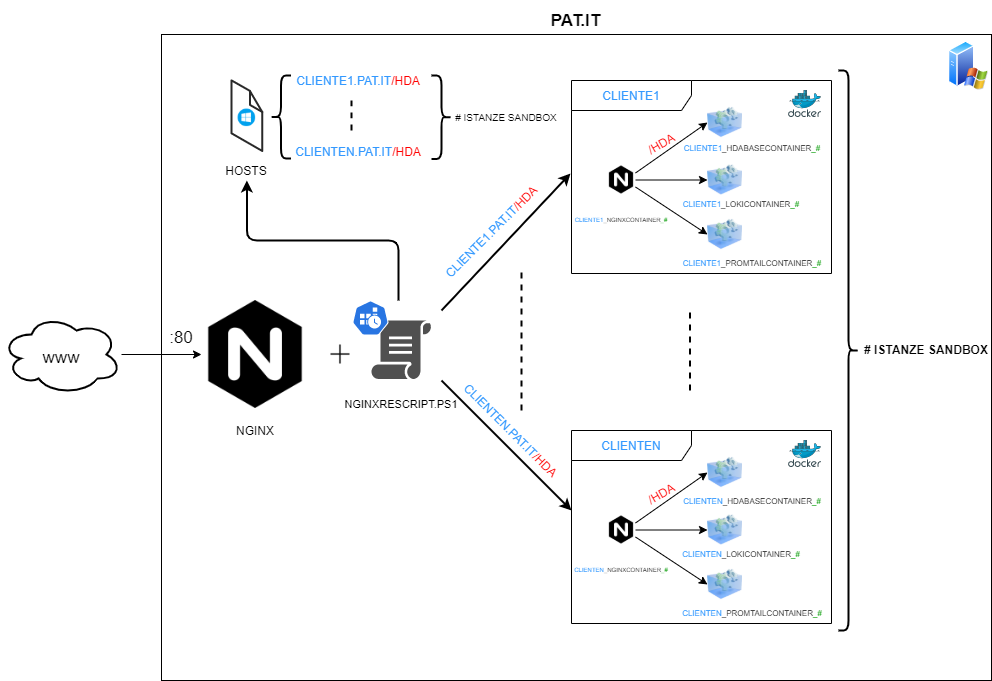
\includegraphics[width=1.0\columnwidth]{immagini/img/hda_containerized_architecture} 
    \caption{Architettura generale del progetto}
\end{figure} 

La figura soprastante rappresenta l'architettura finale del prodotto interamente sviluppata ed installata con successo su un \textit{host}. 
Una sandbox applicativa è un insieme di container in esecuzione, simultaneamente, per un singolo cliente. All'interno di un singolo host possono coesistere multiple \textit{sandbox} applicative, lanciate manualmente dal tecnico installatore.\\
Una \textit{sandbox} applicativa è composta dal seguente insieme di container:
\begin{itemize}
	\item \textbf{nginxcontainer};
	\item \textbf{hdabasecontainer};
	\item \textbf{promtailcontainer};
	\item \textbf{lokicontainer};
\end{itemize}
ed è rappresentata in figura tramite il quadrato contenente appunto i container sopraelencati. Ad ogni \textit{sandbox} è associato un \textbf{nome}, tipicamente proprio del cliente (nell'immagine di esempio ,"cliente1" o "clienten"), ed i container in essa contenuti acquisiscono, nel \textbf{prefisso}, anch'essi il nome della \textit{sandbox}. Ogni cliente sarà associato univocamente ad \textbf{una sola \textit{sandbox} applicativa}, quindi ogni cliente si collegherà solamente alla relativa \textit{sandbox} contenente la versione di HDA (sita nel container "hdabasecontainer") appositamente \textit{customizzata} per lo stesso.
Il corretto instradamento della richiesta dell'utente esterno ad una determinata \textit{sandbox} è gestita dall'istanza di NGINX esterna ad ogni singola sandbox, ma installata nel medesimo \textit{host} (nell'immagine PAT.IT) d'esecuzione delle stesse. All'arrivo di una richiesta esterna HTTP/HTTPS di connessione all'istanza di NGINX esterna attraverso la porta "80" o "443" nel caso di HTTPS, questo controllerà il relativo file di configurazione (nginx.conf) cercando una entry corrispondente al sotto-dominio di primo livello contenuto nel \gls{CNAME} della propria istanza di HDA (ex: \textbf{cliente1}.pat.it) alla quale l'utente vuole collegarsi. Se questa entry (cliente1) è presente all'interno del file "nginx.conf", si instraderà la richiesta all'indirizzo IP, letto nel file "host" del computer "PAT.IT", della relativa \textit{sandbox} appartenente al cliente (la \textit{sandbox} appunto "\textbf{cliente1}.pat.it"). Sarà poi compito dell'istanza di NGINX interna alla \textit{sandbox} (ex: \textbf{cliente1}\_nginxcontainer\_1) instradare la richiesta, precedentemente arrivata dall'istanza NGINX esterna, al relativo container a seconda dei seguenti suffissi:
\begin{itemize}
	\item \textbf{/HDAPortal} instraderà la chiamata al container "hdabasecontainer" e, quindi, all'istanza dell'applicativo HDA contenuto in esso;
	\item \textbf{/loki} instraderà la chiamata al container loki, per la visualizzazione via browser delle metriche di HDA;
	\item \textbf{/promtail} instraderà la chiamata al container "promtailcontainer" contenente un' istanza dell'applicativo "promtail" e si visualizzerà a video una serie di metriche relative all'applicativo HDA.
\end{itemize}
Un eventuale suffisso vuoto "\textbf{/}" instraderà, di default, la chiamata al container "hdabasecontainer".
Il \textit{discovery} di eventuali nuove \textit{sandbox} applicative, o la rimozione di quelle non più attive dal file "host" del sistema operativo, è interamente gestita dallo script Powershell "nginxREscript.ps1". Una panoramica dettagliata relativa alla costruzione e funzionamento di questo script è disponibile al capitolo 6.3 di questo documento.

\section{Composizione container}
Come già precedentemente spiegato in questo documento, un container è un'unità atomica contenente un applicativo con le relative dipendenze atte al suo corretto funzionamento. Ogni container, ad esclusione del container "nginxcontainer" si basa su un'immagine del sistema operativo "Windows ServerCore IIS".\\
La composizione di un container può essere più facilmente espressa tramite la seguente immagine:
\begin{figure}[!h]     
\centering 
    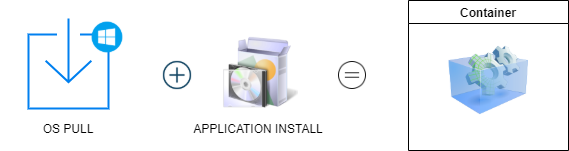
\includegraphics[width=0.5\columnwidth]{immagini/img/container_structure} 
    \caption{Rappresentazione grafica relativa alla composizione generale di un container}
\end{figure} \\
Per necessità progettuali che saranno descritte nel corso di questa relazione è stata necessaria la costruzione di sei diversi container. Di seguito è fornita al lettore una panoramica dettagliata sulla composizione di ognuno dei singoli:\\

\subsection{Container "hdaprepcontainer":}

\begin{namespacedesc}
	\classdesc{S.O./immagine di base} {Windows Servercore IIS}
	\classdesc{Immagine in output} {hdaprepimg}
	\classdesc{Descrizione} {Lo scopo del seguente container è quello di installare una istanza di HDA all'interno di esso, popolando quindi il volume-mapping condiviso con l'host con tutti i file di HDA con i relativi permessi dell'utenza di IIS impostati in automatico dal processo di installazione di HDA lanciato dall'eseguibile "update.exe".
Una volta terminata l'installazione, il container terminerà automaticamente la sua esecuzione. Per lanciare una istanza di HDA containerizzata bisognerà quindi eseguire il successivo container "hdabasecontainer" spiegato immediatamente.}
\end{namespacedesc}
\subsection{Container "hdabasecontainer"}

\begin{namespacedesc}
	\classdesc{S.O./immagine di base} {hdaprepimg}
	\classdesc{Immagine in output}{hdabaseimg}
	\classdesc{Descrizione} {Lo scopo del seguente container è quello di avviare, ed eventualmente re-installare, una istanza di HDA con i relativi servizi. Una volta fatto quanto specificato, a differenza del container hdaprepcontainer, questo non interromperà la sua esecuzione, ma rimarrà attivo per permettere ad utenti esterni di usufruire del programma HDA collegandosi alla web-interface propria dell'istanza di HDA in esecuzione. In aggiunta a questa istanza, è presente una installazione dell'applicativo "Telegraf", atto al monitoraggio in real time dell'istanza di HDA in esecuzione. 
Per favorire uno scambio di dati tra host questo container si interfaccia direttamente con due volume-mapping condivisi con l'host:
\begin{itemize}
	\item \textbf{hdashared}: è il volume-mapping che espone la cartella "App\_Data" del programma HDA. Questo volume-mapping permette all'installatore di esportare od importare degli overrides applicativi per delle customizzazioni specifiche di ogni cliente create ad-hoc dal team di sviluppo sulla base delle esigenze del cliente stesso.
	\item \textbf{lokishared}: è il volume-mapping che espone tutti i log applicativi dell'istanza di HDA, come ad esempio \textit{hda\_log.txt}, \textit{error\_log.txt}, \textit{wsc4\_log.txt}.. al container "lokicontainer" atto al monitoraggio dell'istanza di HDA presente in questo container.
\end{itemize}
Questo container dipende (eredita) il filesystem  ed i relativi permessi precedentemente configurati dal container "hdaprepcontainer".}
\end{namespacedesc}

\subsection{Container "hdadbupdatercontainer"}
\begin{namespacedesc}
	\classdesc{S.O./immagine di base} {hdabaseimg}
	\classdesc{Immagine in output}{hdabasedbimg}
	\classdesc{Descrizione} {Lo scopo del seguente container è quello di eseguire un aggiornamento del database di HDA manualmente creato all'interno di uno specifico server \textbf{MS-SQL}. I parametri di connessione al database pre-esistente di HDA sono nel template-file "istance.json" presente nel pacchetto di installazione di HDA fornito.
Il presente container non ha associato alcun indirizzo IP o scheda di rete virtuale, in quanto l'utente non ha la necessità di interfacciarcisi durante la sua esecuzione e può, inoltre, essere eseguito indipendentemente da qualsiasi altro container in esecuzione sullo stesso host.
La versione di HDA presente nel container "hdaprepcontainer", e di conseguenza nel container "hdabasecontainer", deve essere compatibile con la versione del database installato tramite questo container. Il controllo di versione non è automatizzato, e lo dovrà quindi fare il tecnico installatore manualmente. La tabella informativa relativamente alla compatibilità tra versioni di HDA e database è presente all'interno del file Onenote aziendale.  
}
\end{namespacedesc}

\subsection{Container "lokicontainer"}
\begin{namespacedesc}
	\classdesc{S.O./immagine di base} {Windows Servercore IIS}
	\classdesc{Immagine in output}{lokiimg}
	\classdesc{Descrizione} {Lo scopo del seguente container è quello di eseguire una istanza del programma "Loki" atto al monitoraggio dei servizi di HDA. Il presente container preleva i dati popolati dall'istanza di HDA in esecuzione nel container "hdabasecontainer" nel volume mapping "lokishared"  ad esso collegato, per inviarli direttamente al container "promtailcontainer".}
\end{namespacedesc}

\subsection{Container "promtailcontainer"}
\begin{namespacedesc}
	\classdesc{S.O./immagine di base} {Windows Servercore IIS}
	\classdesc{Immagine in output}{promtailimg}
	\classdesc{Descrizione} {Lo scopo del seguente container è quello di eseguire una istanza del programma "Promtail" atto al monitoraggio dei servizi di HDA in esecuzione sul container "hdabasecontainer". Il seguente container espone i log collezionati dal container "lokicontainer" su una specifica porta precedentemente configurata da apposito file di configurazione "\textit{promtail-local-config.yml"} per permettere all'applicativo "Grafana", in esecuzione su un altro \textit{host} di mostrare graficamente le statistiche ed eventuali errori legati all'istanza di HDA in esecuzione sul container "hdabasecontainer".}
\end{namespacedesc}	

\subsection{Container "nginxcontainer"}
\begin{namespacedesc}
	\classdesc{S.O./immagine di base} {NGINX official image}
	\classdesc{Immagine in output}{nginximg}
	\classdesc{Descrizione} {Lo scopo del seguente container è quello di eseguire una istanza del programma "NGINX" con il relativo file di configurazione "\textit{nginx.conf} automaticamente importato. Tramite il resolver DNS interno di Docker, è possibile per un utente esterno, tramite NGINX, accedere ad un qualsiasi container facente parte della \textit{sandbox} applicativa di HDA, quali "hdabasecontainer", "lokicontainer" e "promtailcontainer". Sempre tramite questo container, è possibile la gestione precedentemente accennata di load-balancing tra molteplici container di HDA.}
\end{namespacedesc}

\newpage	

\section{Dockerfile container: analisi struttura e spiegazione}
Come già visto precedentemente, ogni container è generato da un proprio dockerfile, il quale contiene tutte le istruzioni e comandi atti alla corretta costruzione di una immagine di un applicativo containerizzato.
Di seguito, tramite l'ausilio di \gls{flow-chart} riassuntivi, viene fornita al lettore una panoramica sul contenuto di ogni dockerfile del progetto:
\subsection{Dockerfile container: "hdaprepcontainer"}
Il presente dockerfile costruisce con successo l'immagine relativa al container "hdaprepcontainer". La sequenza di passi per l'ottenimento dell'immagine è di seguito rappresentata:
\begin{figure}[!h]     
\centering 
    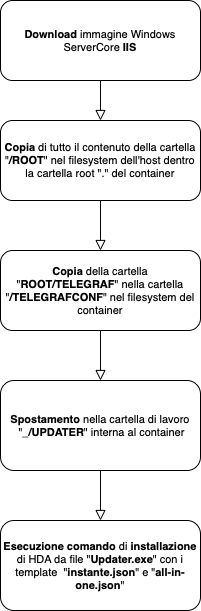
\includegraphics[width=0.3\columnwidth]{immagini/flowchart/flowchart_hdaprepcontainer} 
    \caption{Flow-chart rappresentante la costruzione dell'immagine relativa al container "hdaprepcontainer"}
\end{figure} \\
Questo container non rimane in esecuzione dopo la fine dell'ultima istruzione, e non fa parte della \textit{sandbox} applicativa.\\
\newpage
\subsection{Dockerfile container: "hdadbupdatercontainer"}
Il presente dockerfile costruisce con successo l'immagine relativa al container "hdadbupdatercontainer". La sequenza di passi per l'ottenimento dell'immagine è di seguito rappresentata:
\begin{figure}[!h]     
\centering 
    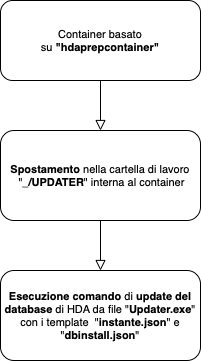
\includegraphics[width=0.3\columnwidth]{immagini/flowchart/flowchart_hdadbinstall} 
    \caption{Flow-chart rappresentante la costruzione dell'immagine relativa al container "hdadbupdatercontainer"}
\end{figure} \\
Questo container non rimane in esecuzione dopo la fine dell'ultima istruzione, e non fa parte della \textit{sandbox} applicativa.\\
\newpage
\subsection{Dockerfile container: "hdabasecontainer"}
Il presente dockerfile costruisce con successo l'immagine relativa al container "hdabasecontainer". La sequenza di passi per l'ottenimento dell'immagine è di seguito rappresentata:
\begin{figure}[!h]     
\centering 
    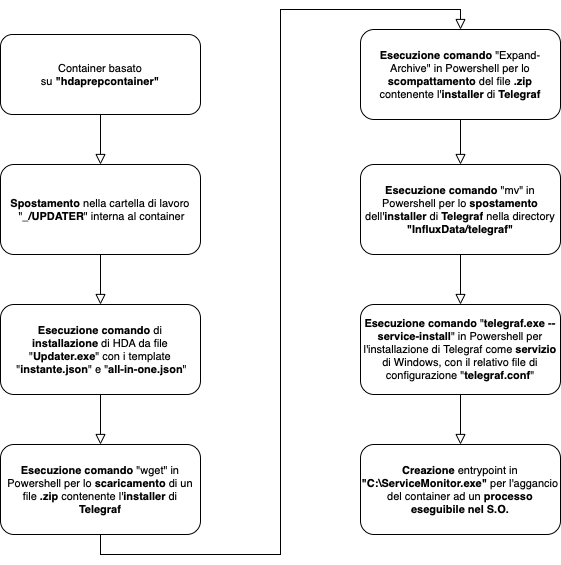
\includegraphics[width=0.7\columnwidth]{immagini/flowchart/flowchart_hdabasecontainer} 
    \caption{Flow-chart rappresentante la costruzione dell'immagine relativa al container "hdabasecontainer"}
\end{figure} \\
Questo container rimane in esecuzione dopo la fine dell'ultima istruzione agganciandosi al processo interno "ServiceMonitor.exe", e fa parte della \textit{sandbox} applicativa.
\newpage
\subsection{Dockerfile container: "lokicontainer"}
Il presente dockerfile costruisce con successo l'immagine relativa al container "lokicontainer". La sequenza di passi per l'ottenimento dell'immagine è di seguito rappresentata:
\begin{figure}[!h]     
\centering 
    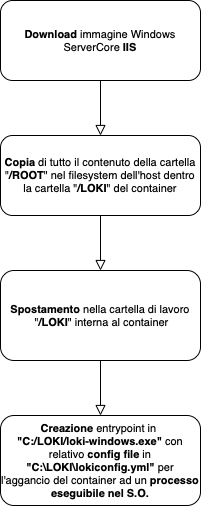
\includegraphics[width=0.3\columnwidth]{immagini/flowchart/flowchart_lokicontainer} 
    \caption{Flow-chart rappresentante la costruzione dell'immagine relativa al container "lokicontainer"}
\end{figure} \\
Questo container rimane in esecuzione dopo la fine dell'ultima istruzione agganciandosi al processo interno "loki-windows.exe", e fa parte della \textit{sandbox} applicativa.
\newpage
\subsection{Dockerfile container: "promtailcontainer"}
Il presente dockerfile costruisce con successo l'immagine relativa al container "promtailcontainer". La sequenza di passi per l'ottenimento dell'immagine è di seguito rappresentata:
\begin{figure}[!h]     
\centering 
    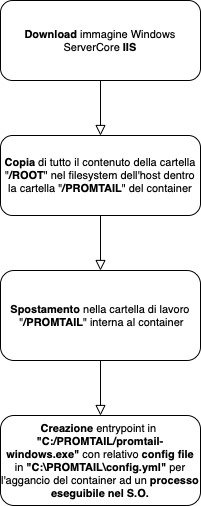
\includegraphics[width=0.3\columnwidth]{immagini/flowchart/flowchart_promtailcontainer} 
    \caption{Flow-chart rappresentante la costruzione dell'immagine relativa al container "promtailcontainer"}
\end{figure} \\
Questo container rimane in esecuzione dopo la fine dell'ultima istruzione agganciandosi al processo interno "promtail-windows.exe", e fa parte della \textit{sandbox} applicativa.
\newpage
\subsection{Dockerfile container: "nginxcontainer"}
Il presente dockerfile costruisce con successo l'immagine relativa al container "nginxcontainer". La sequenza di passi per l'ottenimento dell'immagine è di seguito rappresentata:
\begin{figure}[!h]     
\centering 
    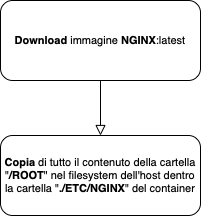
\includegraphics[width=0.3\columnwidth]{immagini/flowchart/flowchart_nginxcontainer} 
    \caption{Flow-chart rappresentante la costruzione dell'immagine relativa al container "nginxcontainer"}
\end{figure} \\
Questo container rimane in esecuzione dopo la fine dell'ultima istruzione, e fa parte della \textit{sandbox} applicativa.
%-------------------------------------



\newpage
\section{Costruzione container tramite automazione: HDA Sandbox Builder}
La costruzione ed il lancio di una \textit{sandbox} applicativa è un'operazione molto onerosa in termini di tempo e di passaggi manuali da eseguire per l'utente installatore.
Per ovviare ad eventuali errori cronologici sul lancio e la costruzione dei container è stato creato un \textit{batch}-file atto al setup ed alla creazione automatizzata dei container, al fine di poter facilmente costruire e lanciare una o più \textit{sandbox} applicative.
Il \textit{batch}-file "\textbf{HDA\_sandbox\_builder.bat}" è uno script-file che consente la creazione ed il setup di HDA nei volume-mapping in maniera totalmente automatizzata, consentendo all'utente installatore la scelta, effettuata tramite risposte \textit{Y/N}, della costruzione delle immagini e dei container stessi.
Il \textit{flow-chart} di esecuzione del batch-file è qui sotto rappresentato:
\\
\begin{figure}[!h]     
\centering 
    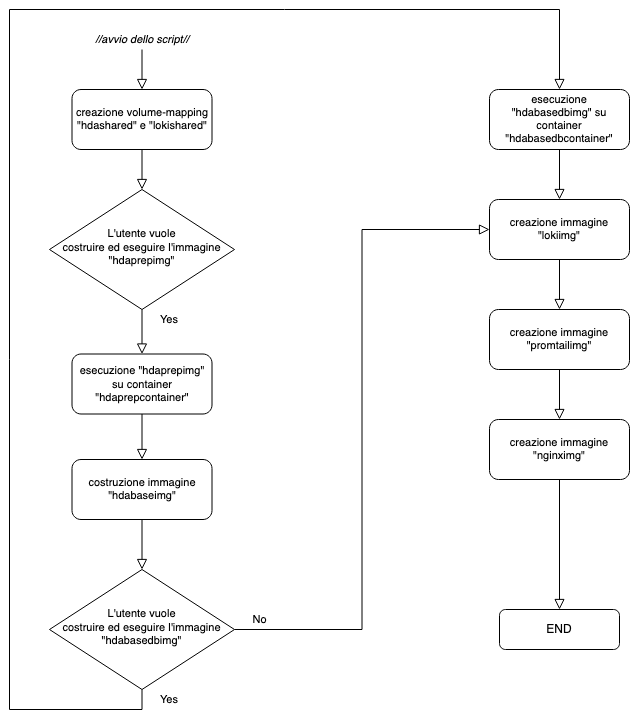
\includegraphics[width=0.8 \columnwidth]{immagini/img/hda_sandbox_builder_fc} 
    \caption{Flow chart del batch-file "hda\_sandbox\_builder.bat"}
\end{figure}\\
Come si evince dal diagramma di flusso, al termine dell'esecuzione del batch-file, non è in esecuzione alcuna \textit{sandbox} applicativa né container. Sono state invece create tutte le immagini applicative sulla quale si baseranno tutti i container propri della \textit{sandbox} applicativa di HDA.
Il lancio dei container veri e propri, e quindi anche della \textit{sandbox} applicativa di HDA, dovrà essere eseguito necessariamente a mano dall'utente installatore o amministratore del server.
Il lancio della \textit{sandbox} applicativa di HDA, grazie ai container appena creati, è ora un'operazione relativamente semplice e veloce, e sarà trattato approfonditamente nella sezione "5.4" di questo documento.
Per favorire al lettore una più corretta comprensione relativamente al batch file \textbf{HDA\_sandbox\_builder.bat} ed alla costruzione dei container, è stato predisposto un diagramma relativo al flusso di esecuzione del \textit{batch}-file con particolare attenzione ai dockerfile e container coinvolti nel flusso di esecuzione dello stesso:
\begin{figure}[!h]     
\centering 
    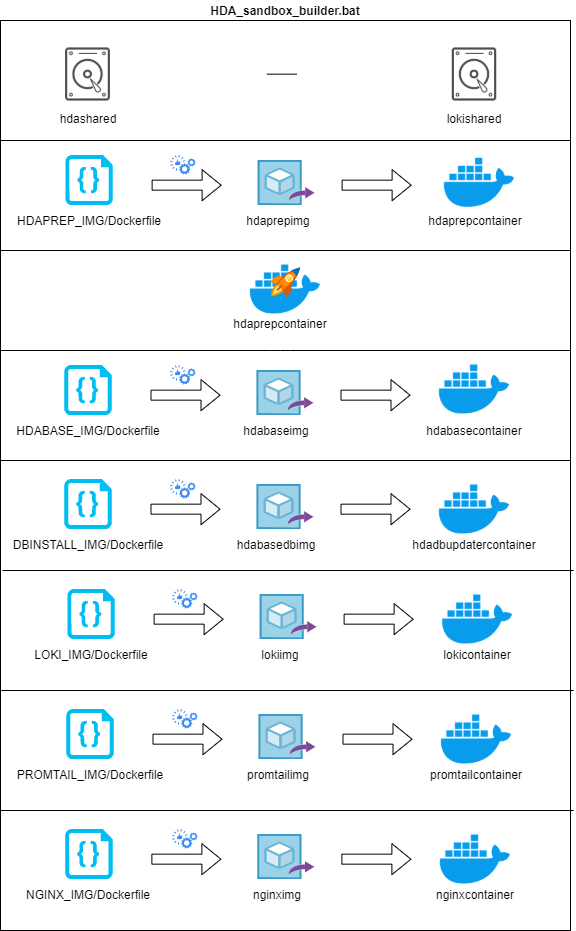
\includegraphics[width=0.7 \columnwidth]{immagini/flowchart/flow_chart_HDA_sandbox_builder} 
    \caption{Flow chart del \textit{batch} file "HDA\_sandbox\_builder.bat" con particolare evidenza ai dockerfile e relativi container coinvolti}
\end{figure}\\
%FLOW CHART ESECUZIONE batch file.
\newpage
\section{Installazione nel computer client}
L'infrastruttura sopracitata, al fine di funzionare correttamente, necessita di una installazione di Docker all'interno del sistema operativo \textit{host} dove verrà creata ed eseguita l'intera infrastruttura.
I passi atti ad una corretta installazione di Docker sono reperibili nella pagina di "Download and Install" nella relativa documentazione di Docker. Un importante accorgimento che l'utente installatore dovrà obbligatoriamente eseguire è lo switching dai container Linux ai container Windows, effettuabile dall'icona di Docker posizionata nella barra Start di Windows, selezionando l'apposita voce "Switch to Windows Containers" come da immagine:
\begin{figure}[!h]     
\centering 
    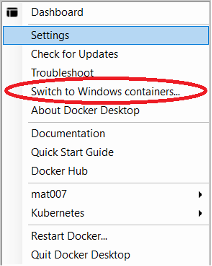
\includegraphics[width=0.2\columnwidth]{immagini/img/switch_windows_container} 
    \caption{Voce da selezionare per cambiare la tipologia di container}
\end{figure}\\
Una volta selezionata la funzionalità sopra riportata, il Docker Engine si riavvierà, permettendo ora la creazione ed esecuzione dei container basati sul sistema operativo Microsoft Windows.\\
Installato con successo l'applicativo Docker, è necessario accedere al file di configurazione dello stesso ("docker.conf") o, tramite Docker Desktop, accedere alle impostazioni dello stesso, per abilitare la funzionalità "experimental features" che permette appunto l'esecuzione su Windows di container basati su Linux (necessario per il container "nginxcontainer"), ed esporre le relative Docker API su una determinata porta.
L'esposizione delle Docker API sono di vitale importanza per l'esecuzione dello script Powershell "nginxREscript.ps1", e la porta precedentemente esposta andrà modificata manualmente anche all'interno dello stesso script.
Il risultato finale sarà simile alla seguente immagine, dove si illustra graficamente, tramite Docker Desktop, il file di configurazione di Docker esponendo le Docker API nella porta "2390":
\begin{figure}[!h]     
\centering 
    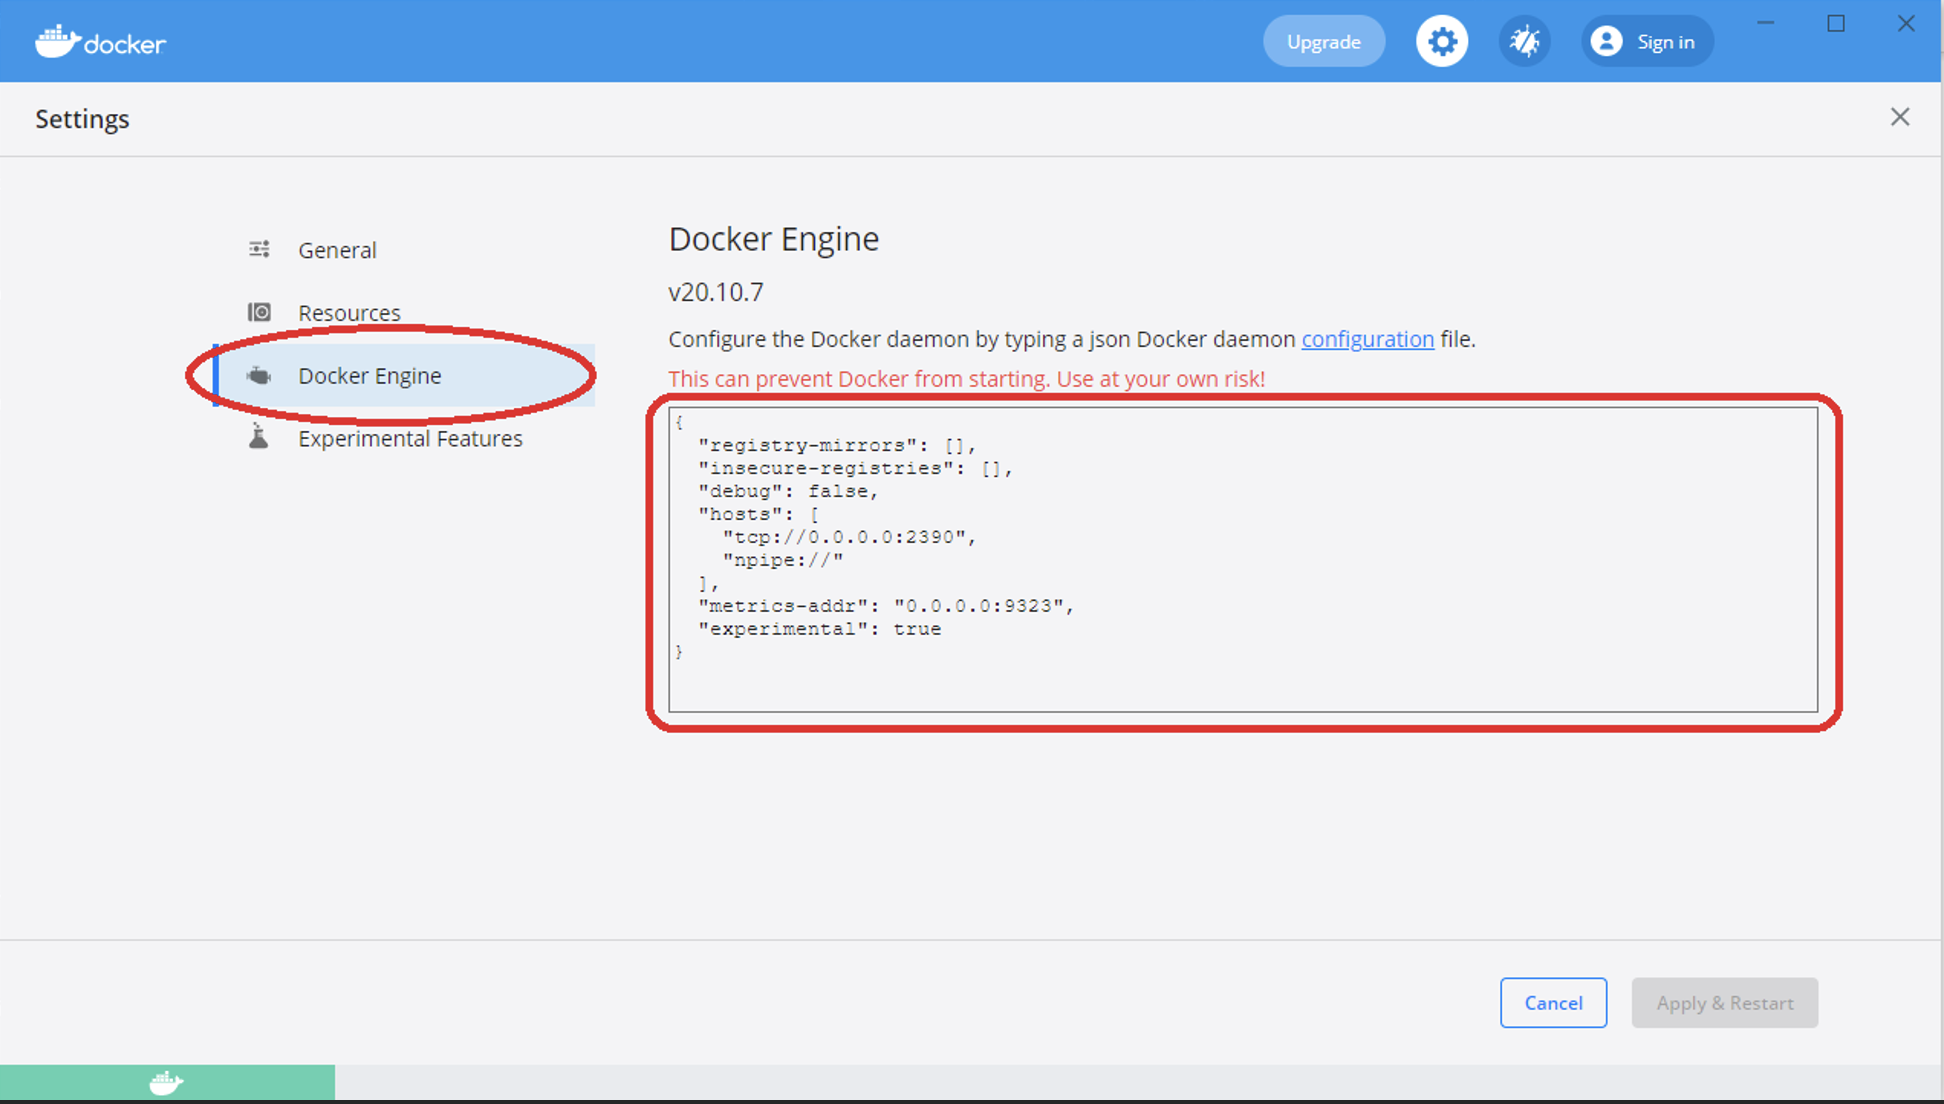
\includegraphics[width=0.7 \columnwidth]{immagini/img/docker_desktop_conf} 
    \caption{File di configurazione di Docker Desktop con le API esposte in porta "2390"}
\end{figure}\\
Ad ogni riavvio della macchina fisica è possibile che Docker Engine vada in errore, in quanto non riuscirà ad esporre le proprie API nella porta precedentemente configurata. Per risolvere questo problema, l'installatore dovrà configurare una nuova porta, non precedentemente utilizzata, esattamente come visto sopra.\\










